\section{Formatowanie}
\label{sec:formatting}

Aby uniknąć nieporozumień dotyczących formatowania poniżej podsumowano najważniejsze informacje jego dotyczące. Czcionki tytułu, i~trzech poziomów zagnieżdżeń sekcji powinny odpowiednio przyjąć rozmiar 14, 12, 10, 10 punktów i~być pogrubione.

\subsection{Podział tekstu}
\label{subsec:textDivision}

W niniejszym przypadku, pierwszy akapit sekcji (niezależnie od poziomu ich zagnieżdżenia) występuje z pominięciem wcięcia.

Następujące po nim akapity powinny być wcięte.

\subsubsection{Poziomy sekcji}
\label{subsubsec:levels}

Zauważmy, że wyłącznie dwa poziomy sekcji są numerowane. Dalsze zagnieżdżenie skutkuje brakiem numeracji - wymagany sposób formatowania tekstu w~tym przypadku to wlewanie nagłówków w~tej samej linii, tak jak opisano w tej sekcji.

\paragraph{Granice zagnieżdżania}
\label{par:nestingLimits}

Pomimo, że szablon LNCS Springer dopuszcza stosowanie czterech poziomów zagnieżdżenia, ostatni poziom najczęściej wpływa negatywnie na czytelność tekstu. Zainteresowany Czytelnik powinien stosować maksymalnie trzy opisywane poziomy, z~pominięciem poziomu zagnieżdżenia tej sekcji. Należy dążyć do rekomendowanej sytuacji, w~której stosowane są dwa poziomy zagnieżdżenia.

\subsubsection{Łamanie linii}
\label{subsubsec:linebreak}

Tekst powinien być wyjustowany. Część wyrazów w~języku polskim (np. krótkie spójniki) nie może być stosowana na końcu linii. Aby tego uniknąć, należy zastosować skrypt porządkujący tekst lub korzystać ze znaku twardej spacji.

\subsubsection{Łamanie stron}
\label{subsubsec:pagebreak}

Dobrą praktyką, nie zawsze możliwą do realizacji, jest przejście do nowej strony na granicach akapitów i~w~taki sposób, aby w treści akapitu kończącego stronę nie było odwołania do ilustracji/tabeli znajdującego się na kolejnej. Należy również unikać kontynuacji niewielkiej części wątku na następnej stronie, szczególnie jeśli jest parzysta (czyli niewidoczna w~trybie czytania dwóch stron jednocześnie).

\subsubsection{Odstępy pionowe}
\label{subsubsec:verticalSpace}

Nadmierne odstępy pionowe utrudniają odbiór tekstu. Próba wdrożenia zasady łamania stron może wpłynąć na zwiększenie tych odstępów - należy unikać takiej sytuacji. Czytelnik jest zobowiązany do przeredagowania tekstu aby była możliwość umieszczenia jeszcze jednego akapitu na stronie, gdy doświadczy opisanego problemu.

\subsection{Uzupełnienia treści}
\label{subsec:additions}

Wśród często stosowanych obiektów urozmaicających treść są tabele i~rysunki. Rozpatrzmy oba przykłady (Tab. \ref{tab:styles}, Rys. \ref{fig:devop}). Zauważmy, że opis powinien znajdować się powyżej tabeli, ale poniżej rysunku. Należy zwrócić uwagę na dopasowanie rozmiaru obiektów do pozostałej treści strony.

\begin{table}
	\vspace{-4mm}
	\caption{
		Style wlewania tekstu.
	}
	\begin{center}
		\begin{tabular}{lll}
			\hline
			Typ & Przykład & Styl i~wielkość czcionki\\
			\hline
			Tytuł & {\Large\bfseries Instrukcja} & 14 punktów, pogrubiona\\
			Sekcja &  {\large\bfseries 1 Wprowadzenie} & 12 punktów, pogrubiona\\
			Podsekcja & {\bfseries 2.1 Podział tekstu} & 10 punktów, pogrubiona\\
			Paragraf & {\bfseries Poziomy sekcji} & 10 punktów, pogrubiona\\
			Zwykły tekst & Nadmierne odstępy pionowe & 10 punktów\\
			\hline
		\end{tabular}
	\end{center}
	\label{tab:styles}
	\vspace{-6mm}
\end{table}

\begin{figure}
	\begin{center}
		\vspace{-5mm}
		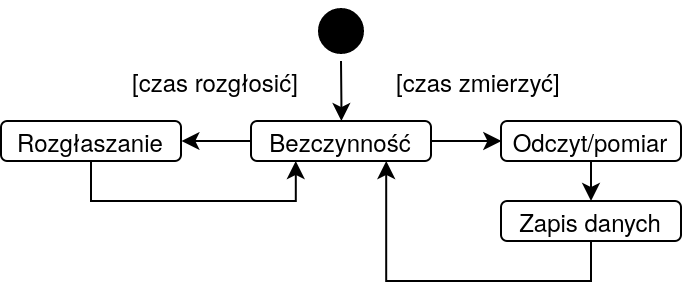
\includegraphics[width=8cm]{device-operation.png}
		\caption{
			Diagram stanów pracy beacona (model uproszczony). Po uruchomieniu i~konfiguracji urządzenie przechodzi w tryb zmniejszonego poboru energii. Operacje rozgłaszania i odczytu/pomiaru są najczęściej wykonywane okresowo.
		}
		\label{fig:devop}
		\vspace{-8mm}
	\end{center}
\end{figure}

\noindent Uzupełnienia treści powinny nawiązywać co najmniej do jednego akapitu sekcji. W~ten sposób Czytelnik jest w stanie poznać intencje autora dotyczące prezentacji obiektów urozmaicających w~artykule. Zbyt krótkie nawiązania mogą być przejawem niedokładności autora tekstu, a zbyt długie - utrudniać zrozumienie jego rozważań.

\subsubsection{Wykresy}
\label{subsubsec:charts}

Korzystając z~tej formy prezentacji informacji, warto pamiętać o~opisaniu osi liczbowych, użyciu adekwatnej skali i~typie wykresu dostosowanym do rodzaju danych, a~także konsekwencji stylistycznej.

\begin{figure}[!h]
	\vspace{-3mm}
	\centering
	\begin{tikzpicture}
		\begin{axis}[
			xlabel={zestaw danych},
			ylabel={rozmiar [b]},
			width=0.9\textwidth,
			height=5.5cm,
			xmin = 1,
			xmax = 90,
			ymax = 85000,
			minor y tick num = 4,
			legend columns=-1
		]
			\addplot table[
				x=lp,y=prop,mark=none
			]{results.csv}; \addlegendentry{propozycja}
			\addplot table[
				x=lp,y=rle,mark=none
			]{results.csv}; \addlegendentry{k. długości serii}
			\addplot table[
				x=lp,y=huffman,mark=none
			]{results.csv}; \addlegendentry{k. Huffmana}
			\draw [dashed] (0, 46080) -- (90, 46080);
		\end{axis}
	\end{tikzpicture}
	\caption{
		Uzyskany rozmiar danych po skorzystaniu z omawianych algorytmów dla zestawów przyrostów wartości liczydła energii czynnej. Linią przerywaną zaznaczono rozmiar przed kompresją. Próba: 90 instalacji na różnych licznikach energii, zbiór danych z~pełnego miesiąca.
	}
	\vspace{-6mm}
	\label{fig:compressionAlgorithms}
\end{figure}

\subsubsection{Wnioskowanie logiczne}
\label{subsubsec:logic}

Pytania, spostrzeżenia, teorie i~hipotezy, lematy, twierdzenia, dowody i wnioski, definicje, przykłady, własności i~rozwiązania - zbiór metodologii zawiera wiele form prezentacji logicznych wyrażeń. Student może je (oszczędnie) stosować, aby uporządkować tok rozumowania.

\begin{claim}
	Każdy wzór matematyczny skraca o~połowę liczbę aktywnych użytkowników prezentacji.
\end{claim}
\begin{proof}
	Załóżmy, że istnieje wzór, który nie skraca liczby aktywnych użytkowników prezentacji o połowę. Przyjmijmy dla ustalenia uwagi, że jest postaci jak poniżej.

	\begin{equation} \label{eq:formula}
	e^{\pi i} + 1 = 0
	\end{equation}

	\noindent Tożsamość Eulera (\ref{eq:formula}), jest uznawana za najpiękniejszy wzór matematyczny z~uwagi na wystąpienie trzech działań arytmetycznych łączących pięć fundamentalnych stałych matematycznych. Ponadto, prezentowane równanie jest wyśrodkowane w~nowej linii (zgodnie ze sztuką). Większość czytelników nadal powinna być skupiona na treści, jednak intuicja podpowiada, że zastanawiają się oni nad sensownością argumentacji, co prowadzi do niespodziewanej sprzeczności. \qed
\end{proof}

Wyciąganie niedokładnych wniosków stanowi o poziomie ignorancji autora. Sugeruje się krytyczne podejście do własnych badań i~intuicji, precyzyjny opis procedury i~środowiska testowego, a~także wnikliwą analizę otrzymanych rezultatów.

\subsubsection{Pseudokod}
\label{subsubsec:pseudocode}

Zaleca się stosowanie pseudokodu aby przedstawić zasadę działania algorytmu. Czytelnik powinien stosować minimalistyczne podejście w~opisie obiektów - jeśli wyłącznie jeden obiekt danego typu występuje, dobrą praktyką jest ukrycie jego numeru, jak na przykładzie poniżej.

\vspace{-4mm}
\begin{algorithm}
	\renewcommand{\thealgorithm}{} % comment it if multiple algorithms exist
	\caption{Algorytm Euklidesa} \label{alg:euclid}
	\begin{algorithmic}[1]
		\Procedure{NWD}{$a,b$} \Comment{Największy wspólny dzielnik liczb a i b}
			\State $r\gets a\bmod b$
			\While{$r\not=0$} \Comment{W przeciwnym przypadku odpowiedź jest trywialna}
				\State $a\gets b$
				\State $b\gets r$
				\State $r\gets a\bmod b$
			\EndWhile \label{alg:euclid:endwhile}
			\State \textbf{return} $b$
		\EndProcedure
	\end{algorithmic}
\end{algorithm}
\vspace{-8mm}

\subsubsection{Cytowanie}
\label{subsubsec:cite}

Preferowanym stylem cytowania są liczby w nawiasach kwadratowych, uporządkowane według kolejności wystąpienia w~artykule \cite{ref:lncs}. Dopuszcza się stosowanie etykiet lub nazwisk, jednak te podejście może wpłynąć negatywnie na czytelność tekstu. Cytowania wielu źródeł powinny być zgrupowane \cite{ref:lncs,ref:latex}, a~wszystkie pozycje literatury - mieć swoje odwołania w tekście.

\subsubsection{Inne konstrukcje}
\label{subsubsec:others}

Zachęca się do niestosowania innych konstrukcji uzupełniających treść, ponieważ mogą one wpłynąć negatywnie na odbiór artykułu przez Czytelnika. Nadużywanie ich w~większości przypadków prowadzi do niezrozumienia treści lub trywializacji zawartości dokumentu.
